\section{Introduction}
\label{sec:intro}

Draw a comb of parallel lines on tracing paper, draw another, lay one over the
other and turn it a few degrees. A third pattern appears: broad, slow bands that
belong to neither sheet, made of ink already on the page and rearranged by
nothing but the small difference between two nearly identical structures.
Moir\'e has been a precision instrument since Rayleigh judged ruled gratings by
the fringes they made against their own copies~\cite{Rayleigh1874Gratings} and
Righi read grating displacement from fringe
motion~\cite{Righi1887Sovrapposizione}. It became an artistic medium in the
1960s~\cite{Oster1963Moire, Oster1965Optical, Seitz1965Responsive}, and artists
have built patterns for it since, by hand~\cite{Watkins1982Kinetic} and by the
plate~\cite{Nicolai2010Index}; it acquired a complete Fourier
theory~\cite{Amidror2009Theory}; it grounded a security-printing
discipline~\cite{Hersch2004Band, Chosson2014Beating}; and it reappeared at the
nanoscale, where two graphene sheets twisted by $1.1^\circ$ form a moir\'e
superlattice whose slow beat reorganizes the material into a
superconductor~\cite{Bistritzer2011Moire, Cao2018Magic}. What it has not become
is a medium an artist can draw in interactively. This paper argues that the
obstacle is a representation, and proposes a different one.

Graphics has related to moir\'e in two nearly disjoint ways. The first is
\emph{suppression}: moir\'e is what undersampling looks like when the signal is
repetitive; essentially the whole of texture filtering exists to prevent
it~\cite{Heckbert1986Survey, Zwicker2002EWA}, and it remains a first-class
concern in neural rendering~\cite{Barron2021MipNeRF}. The second is
\emph{synthesis}, a smaller literature that builds moir\'e on purpose: band
moir\'e images~\cite{Hersch2004Band}, level-line moir\'e~\cite{Chosson2014Beating},
target-driven phase modulation~\cite{Tsai2013Target}, variational layer
design~\cite{Lebanon2001Variational}, artistic
screening~\cite{Ostromoukhov1995Artistic}, micro-optics and curved
fabrication~\cite{Walger2019Moire, Saberpour2020Fabrication}, and, running the
amplification backwards, moir\'e as a sub-millimeter
sensor~\cite{Qiu2023MoireTag, CamposZamora2024MoireWidgets}. Across that second
tradition one assumption is nearly universal: a layer is a rasterized image
of a grating, possibly warped, multiplied against another. Authoring is
therefore offline, since the layers must be solved for and then rasterized;
playback is physical, printed transparencies slid by hand; and the pattern has
a resolution, so displaying it at any other scale can destroy it or invent it
(Figure~\ref{fig:traditions}). Interactive moir\'e toys and prepress suites
exist, but in all of them the fringe is an unmodelled side effect of drawing
two dense patterns; what the literature does not contain, as far as we can
find, is an interactive tool in which the moir\'e itself is represented,
predicted, and stable under zoom. The nearest system,
FabObscura~\cite{Sethapakdi2025FabObscura}, authors barrier-grid occlusion
rather than interference. We think the gap is not a missing feature but a
missing representation.

\begin{figure}[t]
  \centering
  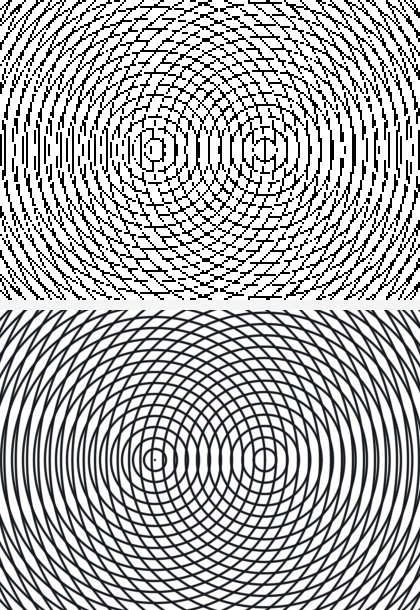
\includegraphics[width=\linewidth]{figures/two-traditions.png}
  \Description{Two square black-on-white panels stacked. Both show two sets of
  concentric rings about different centers, crossing to form a lens-shaped fringe
  pattern. In the upper panel the rings are broken into ragged dashes, the outer rings
  have faded to gray mush, and a coarse blotchy pattern sits over everything. In the
  lower panel every ring is a continuous crisp line right into the corners and the
  only large-scale pattern is the fringe system itself.}
  \caption{\figlead{Raster versus field, same two families.} \emph{Above:} the
  standard synthesis pipeline reused at a scale it was not rasterized for. Each
  layer is rasterized to a bilevel plate, the plates are multiplied, and the
  product is displayed at a different scale, which is what photographing,
  scanning or zooming a printed pair amounts to. (Printed at press resolution and
  viewed in place, the plates never resample; every \emph{screen} reuse of them
  does, and the screen is where an interactive tool lives.) The strokes break into dashes, the
  outer rings dissolve, and a coarse secondary pattern appears that is a property of
  the sampling grid rather than of either family. \emph{Below:} the same two
  families as fields. Two distance queries per pixel, composited, at the display
  resolution. There is no intermediate raster, so the sampling grid contributes
  no pattern of its own, and the crossings stay crisp all the way to the corners.}
  \label{fig:traditions}
\end{figure}

A layer, stripped of its raster, is a countable family of curves
$\{\gamma_n\}$: the $n$th line, the $n$th ring, the $n$th turn of a spiral.
We represent a pattern as a pair $(\cnt,F)$. The \emph{counting map}
$\cnt\colon M\to\T^K$ names the members, fractionally, one coordinate per
family; the \emph{ink} $F$ paints the torus, and the image is $F\circ\cnt$.
The distance field is the leading term of $F$. The index field of a
scalar family is one coordinate of $\cnt$. Superposition is the joint
map. Our central observation is that the interference lives entirely in
$\cnt$: \emph{the visible beat is an integer character $k\cdot\cnt$, and
the fringes are its unit level sets}. Section~\ref{sec:fringe} makes this
precise: the locally averaged ink is a function of $D=\idx_1-\idx_2$
alone, a saturating tent rather than a sinusoid, exact under stated local
hypotheses and first-order accurate beyond them. The same section verifies
the law against $\fringeSamples$ measurements over $\fringeScenes$ pairs of
families, to a mean coverage error of $\fringeMeanErr$.
The locus and the profile shape have classical
ancestors~\cite{Oster1964, Patorski1976Profile, Amidror1994TConv}; what the
counting-map form adds is a per-pixel statement about the actual compositing
operator, with a computable validity criterion: the heterodyne ratio $\het$, a
\emph{field} that can be drawn, telling an author where in the frame a fringe
will form before they commit to parameters. A family's index convention is
arbitrary, so $D$ is one representative of a lattice of integer combinations
$k_1\idx_1+k_2\idx_2$, and the visible moir\'e is whichever combination beats
slowest against the contrast its order costs (\S\ref{sec:visibility}).
Which combination that is turns out to be a best-approximation question
with a classical answer: the visible-beat hierarchy of two pitches is the
continued fraction of their ratio, and in two dimensions the winner is found
exactly, at any order, by per-pixel lattice reduction (\S\ref{sec:selection}).

The catalog sits on an integrability ladder (Section~\ref{sec:object}).
Nine of the thirteen families we ship are exact: parallel lines precomposed
with a field, one line of algebra each. The radial pencil is a defect of
that line family. The families that make the richest interference are the
fold rung. What op artists actually reach for are families whose members
are not concentric: each ring displaced a little further than the last, or
turned a little further, so the family shears, spirals, and finally
unwinds into a pencil of near-parallel curves; Riley's \emph{Blaze}, a nest
of zigzag rings each turned against the last, is exactly such a
family~\cite{Oster1965Optical}. We call these \emph{walking families}
(Section~\ref{sec:walking}): member $n$ is the shape of radius
$ns+\varphi$, displaced by $n\delta$ and turned by $n\theta$. Two extra
parameters, and the closed form is gone. Search is the price of
non-integrability. The obvious search, guess the index from the radius and
check a fixed number of neighbors, fails coherently: the pixels whose true
nearest member falls outside the guessed neighborhood form arcs, not
speckle, so whole sides of whole rings disappear, and the budget is paid at
every pixel whether or not it was needed. For a long time we believed these
broken segments were a rasterization bug; they are an inversion bug.

Section~\ref{sec:inverse} replaces the guess with a certificate. Every radial
metric in this setting (circle, square, triangle, regular $N$-gon) is a
\emph{support function}, and support functions supply exactly the constants the
problem needs: a Lipschitz modulus that lets indices be skipped unevaluated, in
the spirit of sphere tracing~\cite{Hart1996Sphere}; an exact anisotropy floor;
and a subadditive drift rate $\rad(-\delta)$ that is strictly tighter than
$\lVert\delta\rVert$, where using the loose constant declares whole bands of
ordinary settings unsolvable. Together they give a closed interval of integers
that provably contains every member passing within a stroke width of the pixel
(an interval that, unexpectedly, does not involve the rotation $\theta$ at
all) and, when $\theta=0$, a closed form for translated polygons of any side
count, including a marginal case in which the residual is eventually constant
and no enumeration of any finite length can succeed. Measured on the GPU the
certified solver is $\gpuSpeedLo$--$\gpuSpeedHi\times$ faster than the fixed
enumeration it replaces across rotated settings, at equal or better fidelity,
and faster than an exhaustive scan given the same termination bound. Where the
interval genuinely explodes, on the tangent-pencil locus where unboundedly
many members really do crowd a point, Section~\ref{sec:limits} shows the
choice that matters is not how much to subsample but how: anchored to the
family, the error reads as a thinner pattern; anchored to the pixel, as a
shattered one, at identical cost.

\subsection{Contributions}

\begin{itemize}
  \item A counting-map formulation of moir\'e: a pattern is
  $(\cnt,F)$, superposition is a joint torus, and the catalog is an
  integrability ladder of rank times exact / defect / fold
  (Section~\ref{sec:object}). The pattern has no raster at any stage.

  \item The fringe law: locally averaged ink is a saturating tent in the index
  difference, so fringes are its unit level sets. The law is exact under stated
  local hypotheses, per-pixel, with no periodicity assumption, and with a computable
  validity criterion, the heterodyne ratio, drawable as a map
  (Sections~\ref{sec:fringe}--\ref{sec:visibility}).

  \item The selection principle: which beat is visible is best approximation,
  answered by continued fractions in one dimension and by per-pixel
  Lagrange--Gauss reduction of the gradient lattice in two, under an amplitude
  weight that makes ``slowest visible beat'' well posed. The reduction
  replaces an order cap that missed $\selCapMissPct\%$ of visible fringes in
  random carrier pairs, and its winner drives the criterion, the envelope's
  sweep schedule, and the contour overlay (\S\ref{sec:selection}).

  \item Folds and their inversion: walking families, whose index has no
  closed form, and a provably sufficient index interval from the support
  function of the generating shape, a Lipschitz skip rule, and an exact
  closed form for translated polygons of any side count including the
  marginal drift (Section~\ref{sec:inverse}, Appendix~\ref{app:proofs}).

  \item \Moire{}, an interactive tool: thirteen families, twelve concurrent
  layers compiled once, zoom-stable strokes, GPU type morphing, and no
  rasterization step (Section~\ref{sec:system}). Its \emph{envelope} view draws
  the averaged ink directly, which requires averaging over index rather than
  over space; done properly it costs one solve and a few instructions per tap
  rather than one solve per tap (Section~\ref{sec:envelope}).

  \item Moir\'e as a contouring primitive, the corollary of the affine space
  of exact patterns (\S\ref{sec:object}): encoding a scalar field in an
  index difference renders its contours without ever computing a contour.
  The fringes localize to a mean of $\contourWorstErr$\,px of the true
  level sets on the hardest field we tested
  (Section~\ref{sec:beyond}). A circle-valued field mints topological
  defects: fringes that end, with the signed count of endings equal to the
  enclosed winding times the gain, exactly (Section~\ref{sec:defects}).

  \item An expression language for those fields, with the gradient the eikonal
  divide needs obtained by forward-mode differentiation rather than by hand, and
  compiled to straight-line shader code rather than interpreted per pixel. The
  compilation is what makes an arbitrary user-written field affordable:
  $\fieldGainLo$--$\fieldGainHi\times$ cheaper than the interpreter it replaced
  (Section~\ref{sec:exprs}).
\end{itemize}
